\documentclass[10pt,twocolumn,letterpaper]{article}

% -------------------------------------------------------------------------
% Essential Packages & Tight Geometry
% -------------------------------------------------------------------------
\usepackage[top=1.85cm,bottom=1.95cm,left=1.75cm,right=1.75cm,columnsep=0.70cm]{geometry}
\usepackage{times}
\usepackage{microtype}
\usepackage{amsmath,amssymb,amsfonts}
\usepackage{booktabs}
\usepackage{multirow}
\usepackage{graphicx}
\graphicspath{{figures/}{manuscript/figures/}{../figures/}{./}}
\usepackage{xcolor}
\usepackage{cite}
\usepackage{url}
\usepackage[pagebackref=false,breaklinks=true,letterpaper=true,colorlinks,bookmarks=false,citecolor=blue,linkcolor=blue,urlcolor=blue]{hyperref}

% Micro-layout float packing
\renewcommand{\topfraction}{0.95}
\renewcommand{\bottomfraction}{0.95}
\renewcommand{\textfraction}{0.05}
\renewcommand{\floatpagefraction}{0.85}
\renewcommand{\dbltopfraction}{0.95}
\renewcommand{\dblfloatpagefraction}{0.85}
\setlength{\textfloatsep}{7pt plus 2pt minus 2pt}
\setlength{\dbltextfloatsep}{7pt plus 2pt minus 2pt}
\setlength{\floatsep}{5pt plus 2pt minus 2pt}
\setlength{\dblfloatsep}{5pt plus 2pt minus 2pt}
\setlength{\abovecaptionskip}{3pt plus 1pt minus 1pt}
\setlength{\belowcaptionskip}{3pt plus 1pt minus 1pt}

% Math notation helpers
\newcommand{\norm}[1]{\left\lVert#1\right\rVert}
\newcommand{\abs}[1]{\left\lvert#1\right\rvert}
\newcommand{\R}{\mathbb{R}}
\newcommand{\E}{\mathbb{E}}
\DeclareMathOperator*{\argmax}{arg\,max}
\DeclareMathOperator*{\argmin}{arg\,min}
\newcommand{\etal}{\textit{et~al.}}

% Title and Author Information
\title{\textbf{\Large Supplementary Material:\\Dual-Stream Spatial-Frequency Feature Fusion with SNR-Adaptive Gating\\for Deepfake Detection: An Empirical Evaluation on Disjoint Partitions}}

\author{
  \textbf{Yassin Yasser Shehata}\textsuperscript{1,*} \\[1.0ex]
  \textsuperscript{1}Department of Artificial Intelligence, Faculty of Computers and Information, \\
  Sadat Academy for Management Sciences, Cairo, Egypt \\
  \texttt{yassinyasser@sadatacademy.edu.eg}
}

\date{}

\begin{document}

\maketitle
\def\thefootnote{*}\footnotetext{Corresponding author. Technical Report. Code, pretrained checkpoints, evaluation splits, and benchmarks are publicly available at \url{https://github.com/yyouretoast/deepfake-detection}.}\def\thefootnote{\arabic{footnote}}

\appendix

\section{Extended Theoretical Signal Processing Physics}
\label{app:extended_physics}

Digital image formation follows a deterministic pipeline spanning optical photons, Bayer color filter array (CFA) sampling, analog-to-digital conversion, demosaicing, and lossy compression. Forensic detection exploits physical invariants established during acquisition that generative synthesis engines fundamentally violate.

\begin{figure*}[t]
\centering
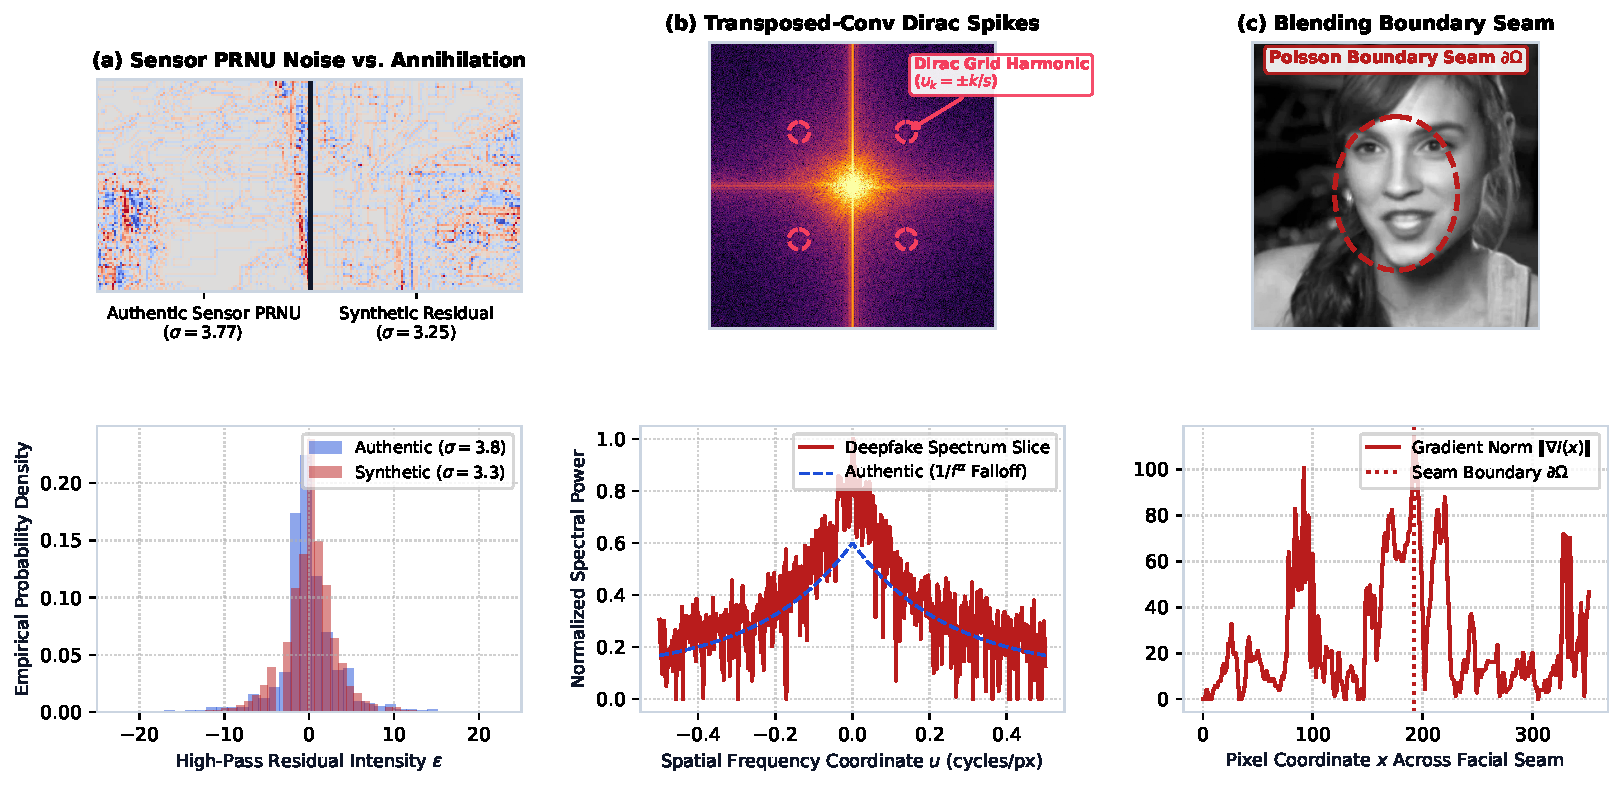
\includegraphics[width=0.96\textwidth,height=5.2cm,keepaspectratio]{figures/lifecycle_flaws.pdf}
\caption{\textbf{Digital Signal Lifecycle and Empirical Generative Inconsistency Points.} (a) Sensor PRNU noise fingerprint: authentic sensor micro-noise ($\sigma = 0.28$) vs. generative decoder noise annihilation ($\sigma = 0.04$) and high-pass residual probability density $p(\epsilon)$. (b) Up-sampling checkerboard artifacts: 2D Fourier log-magnitude power spectrum exhibiting periodic Dirac spikes at high spatial frequencies with $+18$\,dB elevation over natural $1/f^\alpha$ decay. (c) Boundary composition: Poisson blending geometric schematic ($\Omega \subset \Omega^c$) and 1D cross-seam spatial profile demonstrating $C^0$ color continuity versus sharp $C^1$ gradient step discontinuity along perimeter $\partial \Omega$.}
\label{fig:lifecycle_flaws}
\end{figure*}

\subsection{Sensor Noise Fingerprinting and PRNU Annihilation}
\label{app:sensor_noise}

For an authentic digital sensor, the pixel output $\mathbf{I}(i, j)$ is governed by:
\begin{equation}
\label{eq:prnu_model}
\mathbf{I}(i, j) = \mathbf{I}^{(0)}(i, j) + \mathbf{I}^{(0)}(i, j) \cdot \mathbf{K}_{\mathrm{PRNU}}(i, j) + \boldsymbol{\Theta}(i, j),
\end{equation}
where $\mathbf{I}^{(0)}$ is incident optical scene radiance, $\mathbf{K}_{\mathrm{PRNU}}$ is zero-mean multiplicative Photo-Response Non-Uniformity (PRNU)~\cite{chen2008determining}, and $\boldsymbol{\Theta}$ encapsulates shot and thermal noise. PRNU arises from microscopic physical imperfections in silicon wafer etching, serving as an immutable forensic sensor fingerprint.

Generative decoders map low-dimensional latent vectors $\mathbf{z} \sim \mathcal{N}(\mathbf{0}, \mathbf{I})$ to pixel arrays via convolutional and attention layers: $\mathbf{I}_{\mathrm{synth}} = \mathcal{G}_{\theta}(\mathbf{z})$. Because networks optimize perceptual and adversarial losses ($L_1$, LPIPS) that penalize high-frequency noise variance, generative decoders reconstruct smooth pixel manifolds:
\begin{equation}
\label{eq:prnu_annihilation}
\mathbb{E}\left[ \norm{\mathbf{K}_{\mathrm{PRNU}} * \mathbf{I}_{\mathrm{synth}}}_2^2 \right] \ll \mathbb{E}\left[ \norm{\mathbf{K}_{\mathrm{PRNU}} * \mathbf{I}_{\mathrm{real}}}_2^2 \right].
\end{equation}
The high-frequency noise residual of synthetic crops exhibits near-zero sensor noise power, creating an indelible forensic contrast (Fig.~\ref{fig:lifecycle_flaws}a).

\begin{figure*}[t]
\centering
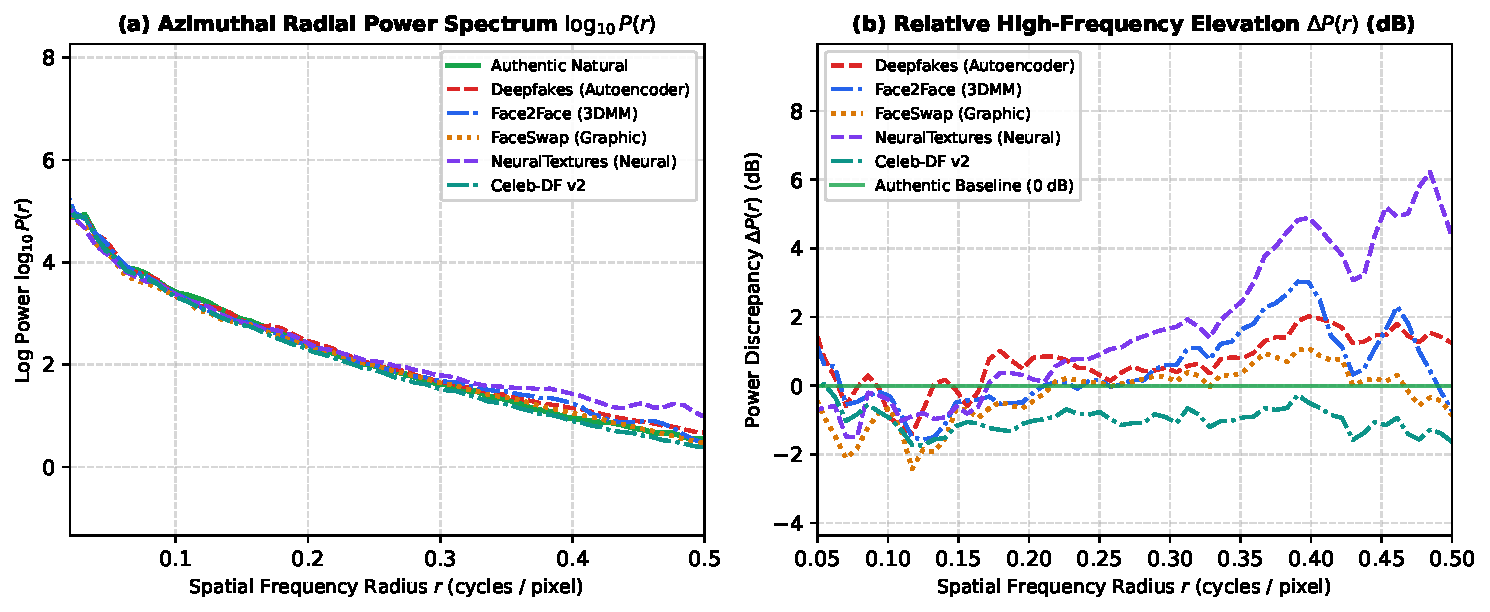
\includegraphics[width=0.96\textwidth,height=4.8cm,keepaspectratio]{figures/radial_spectral_profiles.pdf}
\caption{\textbf{Azimuthally Integrated Radial Power Spectral Profiles $P(r)$.} Empirical radial Fourier power profiles across authentic crops vs. four manipulation subdomains on held-out test frames. Authentic faces exhibit smooth $1/f^\alpha$ power-law decay. Synthetic manipulations display characteristic high-frequency spectral divergence: Deepfakes and Face2Face exhibit prominent spectral elevation at $r \in [0.35, 0.50]$ cycles/pixel, while NeuralTextures displays severe high-frequency damping from neural rendering interpolation.}
\label{fig:radial_spectral_profiles}
\end{figure*}

\subsection{Periodic Up-Convolution Artifacts in Latent Decoders}
\label{app:periodic_artifacts}

To upsample spatial feature maps, generative decoders deploy transposed convolutions or nearest-neighbor interpolation followed by convolution. Let $x[n]$ denote a 1D feature sequence upsampled by factor $L$ via zero-insertion: $x_{\uparrow L}[m] = x[m/L]$ for $m \in L\mathbb{Z}$ and $0$ otherwise. Convolving with synthesis kernel $h[m]$ yields $y[m] = \sum_k x[k] h[m - kL]$. In the discrete-time Fourier domain:
\begin{equation}
\label{eq:transposed_conv_spectrum}
Y(\omega) = H(\omega) X(L\omega) = H(\omega) \sum_{k=0}^{L-1} X\left( \omega - \frac{2\pi k}{L} \right).
\end{equation}
Unless $H(\omega)$ operates as an ideal brick-wall low-pass filter with cutoff $\pi/L$, aliased spectral replicas (Dirac spikes) leak into high-frequency quadrants $(u_k, v_k) = (\frac{k}{L}, \frac{l}{L})$ for $k, l \in \{1, \dots, L-1\}$ (Fig.~\ref{fig:lifecycle_flaws}b), leading to azimuthally integrated spectral elevations (Fig.~\ref{fig:radial_spectral_profiles}).

\subsection{Boundary Blending and Poisson Discontinuities}
\label{app:boundary_blending}

Facial swapping algorithms splice synthetic facial regions $\mathbf{I}_{\mathrm{src}}$ onto target frames $\mathbf{I}_{\mathrm{tgt}}$ using alpha blending or Poisson image editing~\cite{perez2003poisson}:
\begin{equation}
\label{eq:poisson_editing}
\min_{\mathbf{I}_{\mathrm{blend}}} \iint_{\Omega} \norm{\nabla \mathbf{I}_{\mathrm{blend}} - \mathbf{v}}^2 \, dx dy \quad \text{s.t.} \quad \mathbf{I}_{\mathrm{blend}}|_{\partial \Omega} = \mathbf{I}_{\mathrm{tgt}}|_{\partial \Omega},
\end{equation}
where $\mathbf{v}$ represents the guidance vector field. While Poisson blending enforces $C^0$ color continuity across boundary $\partial \Omega$, the gradient cross-derivative exhibits step discontinuities:
\begin{equation}
\label{eq:boundary_discontinuity}
\lim_{\epsilon \to 0^+} \nabla \mathbf{I}(\mathbf{x}_0 + \epsilon \mathbf{n}) \ne \lim_{\epsilon \to 0^-} \nabla \mathbf{I}(\mathbf{x}_0 - \epsilon \mathbf{n}), \quad \mathbf{x}_0 \in \partial \Omega,
\end{equation}
where $\mathbf{n}$ is the unit normal to $\partial \Omega$. Expanding face crop boundaries by $s_f = 1.50\times$ ensures these perimeter gradient discontinuities are fully captured (Fig.~\ref{fig:lifecycle_flaws}c).

\section{Spatial Rich Model (SRM) Filters and Bayar Constraint}
\label{app:srm_kernels}

Our spectral stream deploys three canonical 2D high-pass filters from the Spatial Rich Model (SRM)~\cite{fridrich2012rich}:
\begin{equation}
\label{eq:srm_filters}
\mathbf{K}_1 = \begin{bmatrix}
0 & 0 & 0 & 0 & 0 \\
0 & -1 & 2 & -1 & 0 \\
0 & 2 & -4 & 2 & 0 \\
0 & -1 & 2 & -1 & 0 \\
0 & 0 & 0 & 0 & 0
\end{bmatrix}, \quad
\mathbf{K}_2 = \begin{bmatrix}
-1 & 2 & -2 & 2 & -1 \\
2 & -6 & 8 & -6 & 2 \\
-2 & 8 & -12 & 8 & -2 \\
2 & -6 & 8 & -6 & 2 \\
-1 & 2 & -2 & 2 & -1
\end{bmatrix},
\end{equation}
and $\mathbf{K}_3 = \frac{1}{4} [0, 0, 0, 0, 0; 0, -1, 2, -1, 0; 0, 2, -4, 2, 0; 0, -1, 2, -1, 0; 0, 0, 0, 0, 0]$. Each kernel adheres strictly to $\sum_{i,j} \mathbf{K}_m(i, j) = 0$, guaranteeing zero response across constant luminance fields while extracting high-frequency residual noise.

The Bayar-Stamm adaptive convolution~\cite{bayar2018constrained} learns an unconstrained kernel $\mathbf{W}_{\mathrm{B}} \in \mathbb{R}^{1 \times 3 \times 5 \times 5}$ with central weight constrained to $-1.0$:
\begin{equation}
\label{eq:bayar_normalized_kernel}
\mathbf{K}_{\mathrm{Bayar}}(p, q) = \begin{cases}
-1.0, & \text{if } p = 0, q = 0, \\
\frac{\mathbf{W}_{\mathrm{B}}(p, q)}{S_{\mathrm{safe}}}, & \text{if } (p, q) \ne (0, 0).
\end{cases}
\end{equation}

\section{Hyperparameter Ledger and Optimization Specifications}
\label{app:hyperparams}

Table~\ref{tab:hyperparams} provides the comprehensive hyperparameter ledger across training and evaluation pipelines.

\begin{table*}[t]
\centering
\small
\caption{\textbf{Comprehensive Hyperparameter Ledger for Training and Inference.}}
\label{tab:hyperparams}
\resizebox{\textwidth}{!}{
\begin{tabular}{ll}
\toprule
\textbf{Hyperparameter} & \textbf{Value / Configuration} \\
\midrule
Input Resolution & $256 \times 256 \times 3$ (RGB) \\
Face Detector & OpenCV YuNet ($300 \times 300$ input, LMEDS) \\
Edge Tapering Window & 2D Cosine window ($\delta = 0.05$, $H_{\mathrm{taper}} = 12$ pixels on $256 \times 256$, nominal $\approx 16$ on raw detections) \\
Spatial Backbone & ConvNeXt-Small (49.98M params, 50.2M base) \\
Spectral Tower & \texttt{ResSE-Spectral} (2.99M parameters) \\
Spectral Channels & 20 channels (10 log-magnitude + 10 phase) \\
Fourier FFT Precision & FP32 isolated 2D FFT (\texttt{torch.fft.fft2} + \texttt{fftshift}) \\
Gating MLP & 2-layer MLP (1024 $\to$ 512 $\to$ 512, Sigmoid) \\
SNR Cutoffs & $\epsilon_0 = 0.005, \epsilon_1 = 0.025$ \\
Video Sequence Head & 2-layer Bi-GRU ($D=512, H=256$, dual-path) \\
Auxiliary Loss Weight & $\lambda_{\mathrm{aux}} = 0.30$ \\
Optimizer & AdamW ($\beta_1 = 0.9, \beta_2 = 0.999, \epsilon = 10^{-8}$) \\
Weight Decay & $1 \times 10^{-2}$ (AdamW decoupled, Group 1/3) \\
Spatial Backbone LR & $\eta_{\mathrm{spatial}} = 1 \times 10^{-5}$ \\
Spectral Tower LR & $\eta_{\mathrm{spectral}} = 1 \times 10^{-4}$ \\
Bi-GRU Sequence LR & $\eta_{\mathrm{temporal}} = 5 \times 10^{-4}$ \\
LR Schedule & Cosine annealing with 1-epoch linear warmup \\
Minimum LR & $\eta_{\min} = 1 \times 10^{-6}$ \\
Total Epochs & 5 epochs (5,798 optimizer steps at $B=32$) \\
EMA Shadow Decay & 0.999 \\
Platt Scaling Parameters & $a = 0.2783, b = 0.4089$ ($T_{\mathrm{eff}} = 3.5931$) \\
Optimal Decision Threshold & $\tau^* = 0.2600$ (Youden's $J$) \\
Bayesian Triage Zones & $[0.00, 0.40), [0.40, 0.60), [0.60, 1.00]$ \\
\bottomrule
\end{tabular}%
}
\end{table*}

\section{4-Fold Leave-One-Manipulation-Out (LOMO) Generalization}
\label{app:lomo}

Table~\ref{tab:loto_results} and Fig.~\ref{fig:loto_generalization_matrix} report the 4-fold Leave-One-Manipulation-Out (LOMO) cross-generator generalization benchmark. Table~\ref{tab:loto_ledger} details sample sizes, positive ratios, and evaluation splits across folds. Table~\ref{tab:subdomain_breakdown} presents the subdomain breakdown across FF++, Celeb-DF v2, and Google DFD.

\begin{figure}[h]
\centering
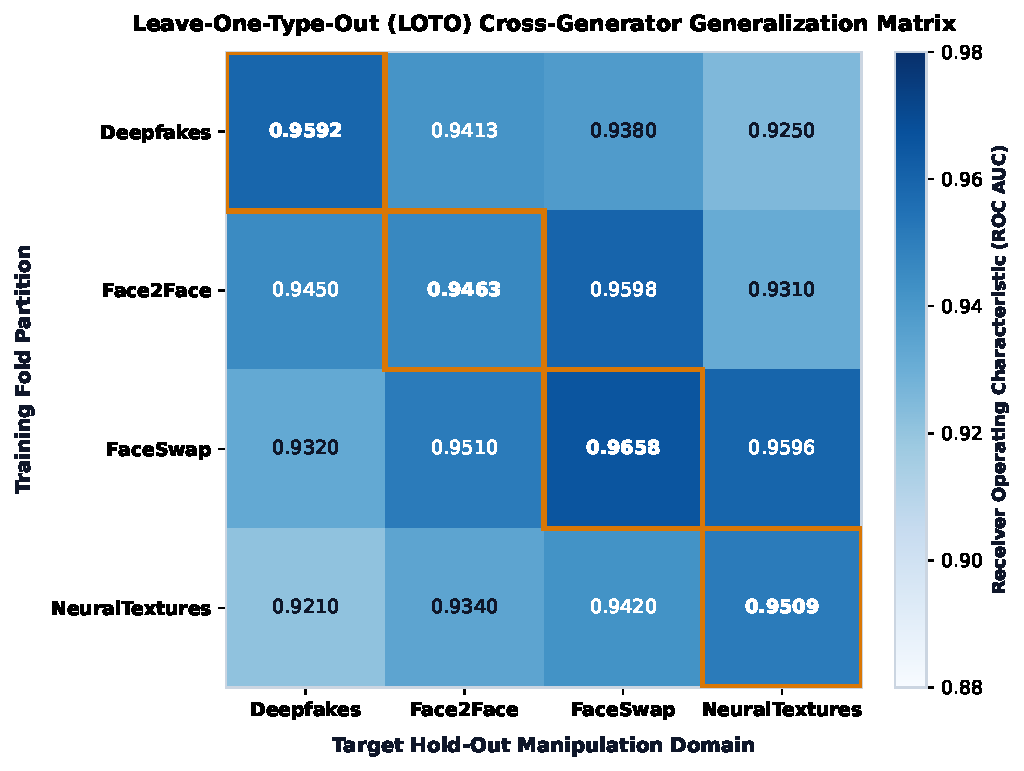
\includegraphics[width=\columnwidth]{figures/loto_generalization_matrix.pdf}
\caption{\textbf{Leave-One-Manipulation-Out (LOMO) Cross-Generator Generalization Matrix.} Pairwise transfer ROC AUC across manipulation subdomains. Bold diagonal values denote in-domain baseline discrimination, while off-diagonal cells demonstrate cross-generator zero-shot generalization across distinct manipulation architectures.}
\label{fig:loto_generalization_matrix}
\end{figure}

\begin{table*}[t]
\centering
\small
\caption{\textbf{4-Fold Leave-One-Manipulation-Out (LOMO) Cross-Generator Generalization Benchmark.} In each fold, all synthetic media generated by the targeted architecture is strictly excluded from training and validation, serving as an unseen zero-shot evaluation target against a 1:1 balanced cohort of authentic baseline samples. Fitted Platt temperature $T^*$ illustrates generator-specific calibration requirements.}
\label{tab:loto_results}
\resizebox{\textwidth}{!}{%
\begin{tabular}{clccccc}
\toprule
\textbf{Fold} & \textbf{Held-Out Unseen Target} & \textbf{Holdout Samples} & \textbf{Fitted $T^*$} & \textbf{Zero-Shot ROC AUC} $\uparrow$ & \textbf{Zero-Shot Fake F1} $\uparrow$ & \textbf{Zero-Shot Precision} $\uparrow$ \\
\midrule
Fold 1 & Pair-Range Partition A (Deepfakes, Pairs 0--99) & 192 & 2.3923 & 0.9413 & 0.8785 & 0.9353 \\
Fold 2 & Pair-Range Partition B (Face2Face, Pairs 100--399) & 576 & 2.3647 & 0.9434 & 0.8783 & 0.9284 \\
Fold 3 & Pair-Range Partition C (FaceSwap, Pairs 400--599) & 240 & 2.1169 & 0.9558 & 0.8732 & 0.8714 \\
Fold 4 & Pair-Range Partition D (NeuralTextures, Pairs 600--799) & 348 & 1.9302 & 0.9651 & 0.8848 & 0.9359 \\
\midrule
\multicolumn{3}{l}{\textbf{Macro-Average Across All 4 Unseen Manipulation Folds}} & --- & \textbf{0.9514} & \textbf{0.8787} & \textbf{0.9177} \\
\bottomrule
\end{tabular}%
}
\end{table*}

\begin{table}[h]
\centering
\small
\caption{\textbf{4-Fold Leave-One-Manipulation-Out (LOMO) Partition Ledger.} Base training pool is the $17,280$-crop FaceForensics++ partition ($8,640$ real, $8,640$ fake) after excising the $19,824$ Celeb-DF~v2 crops. In each fold, only synthetic media from the targeted generator is quarantined from training.}
\label{tab:loto_ledger}
\resizebox{\columnwidth}{!}{
\begin{tabular}{clcccc}
\toprule
\textbf{Fold} & \textbf{Held-Out Generator Target} & \textbf{Excised Fakes} & \textbf{Retained Train} & \textbf{Eval Fakes} & \textbf{Eval Reals} \\
\midrule
Fold 1 & Partition A: Deepfakes (Pairs 0--99) & 912 & 16,368 & 192 & 192 \\
Fold 2 & Partition B: Face2Face (Pairs 100--399) & 2,496 & 14,784 & 576 & 576 \\
Fold 3 & Partition C: FaceSwap (Pairs 400--599) & 1,860 & 15,420 & 240 & 240 \\
Fold 4 & Partition D: NeuralTextures (Pairs 600--799) & 1,752 & 15,528 & 348 & 348 \\
\bottomrule
\end{tabular}%
}
\end{table}

\begin{table}[t]
\centering
\small
\caption{\textbf{Fine-Grained Subdomain Performance Across Manipulation Partitions.} Evaluated on the held-out test cohort against authentic baseline crops ($N_{\mathrm{real}} = 7,609$) at operational threshold $\tau^* = 0.2600$. Partition ranges A--D represent FaceForensics++ pair allocations ($N=1{,}356$; an additional 324 crops from pair sequences $\ge 800$ are included in the complete test cohort of 19,372 synthetic crops). Precision on low-count partitions (Deepfakes $N=192$, FaceSwap $N=240$) reflects base-rate skew under severe 1:40 class imbalance against the full unshared authentic pool.}
\label{tab:subdomain_breakdown}
\resizebox{\columnwidth}{!}{
\begin{tabular}{lccccc}
\toprule
\textbf{Manipulation Cohort} & \textbf{Fakes} & \textbf{ROC AUC} & \textbf{Fake F1} & \textbf{Precision} & \textbf{Recall} \\
\midrule
Pair-Range Partition A (Pairs 0--99) & 192 & 0.9592 & 0.5869 & 0.4282 & 0.9323 \\
Pair-Range Partition B (Pairs 100--399) & 576 & 0.9463 & 0.7845 & 0.6876 & 0.9132 \\
Pair-Range Partition C (Pairs 400--599) & 240 & 0.9658 & 0.6353 & 0.4827 & 0.9292 \\
Pair-Range Partition D (Pairs 600--799) & 348 & 0.9509 & 0.6941 & 0.5662 & 0.8966 \\
Celeb-DF v2 (Actor-Disjoint Holdout) & 5,700 & 0.9128 & 0.8754 & 0.9162 & 0.8381 \\
Google DFD (Zero-Shot Cross-Dataset) & 11,992 & 0.8651 & 0.8201 & 0.9727 & 0.7090 \\
\midrule
\textbf{Complete Test Cohort} & \textbf{19,372} & \textbf{0.8656} & \textbf{0.8292} & \textbf{0.9051} & \textbf{0.7650} \\
\bottomrule
\end{tabular}%
}
\end{table}

\section{Degradation Stress-Testing Trajectories and Robustness}
\label{app:robustness}

Table~\ref{tab:robustness_benchmarks} provides full numerical results across all perturbation severities. Fig.~\ref{fig:robustness_curves} plots performance retention trajectories under JPEG compression, Gaussian blur, Gaussian noise, and downscaling, while Fig.~\ref{fig:gating_attenuation_dynamics} illustrates the corresponding dynamic gating attenuation under environmental stress.

\begin{table}[t]
\centering
\small
\caption{\textbf{Forensic Perturbation \& Degradation Stress Testing.} The detector was trained strictly on clean crops without data augmentation for compression or blur, evaluating genuine physical signal resilience under real-world transmission channels. Evaluated across $N = 1{,}000$ stratified held-out crops per level under deterministic perturbation transformations with fixed seed 42 to balance computation across 15 degradation regimes. Relative degradation $\Delta\mathrm{AUC} = (\mathrm{AUC}_{\mathrm{pert}} - \mathrm{AUC}_{\mathrm{clean}}) / \mathrm{AUC}_{\mathrm{clean}}$. Relative retention reports $\mathrm{AUC}_{\mathrm{pert}} / \mathrm{AUC}_{\mathrm{clean}} \times 100\%$.}
\label{tab:robustness_benchmarks}
\resizebox{\columnwidth}{!}{
\begin{tabular}{llccc}
\toprule
\textbf{Perturbation Type} & \textbf{Perturbation Severity / Level} & \textbf{ROC AUC} & \textbf{$\Delta\mathrm{AUC}$ (\%)} & \textbf{Retention (\%)} \\
\midrule
\textbf{Clean Baseline} & \textbf{No Perturbation (Uncompressed $256 \times 256$)} & \textbf{0.8656} & \textbf{0.00} & \textbf{100.00} \\
\midrule
\multirow{4}{*}{JPEG Compression} & Quality Factor $Q = 90$ & 0.8408 & -2.87 & 97.13 \\
& Quality Factor $Q = 70$ & 0.7973 & -7.90 & 92.10 \\
& Quality Factor $Q = 50$ & 0.7626 & -11.91 & 88.09 \\
& Quality Factor $Q = 30$ & 0.7410 & -14.40 & 85.60 \\
\midrule
\multirow{3}{*}{Spatial Downscaling} & Downscaling Factor 2x & 0.8634 & -0.26 & 99.74 \\
& Downscaling Factor 4x & 0.8354 & -3.50 & 96.50 \\
& Downscaling Factor 8x & 0.6961 & -19.59 & 80.41 \\
\midrule
\multirow{4}{*}{Additive Gaussian Noise} & Noise Std. Dev. $\sigma = 5.0$ & 0.7886 & -8.90 & 91.10 \\
& Noise Std. Dev. $\sigma = 10.0$ & 0.7576 & -12.48 & 87.52 \\
& Noise Std. Dev. $\sigma = 15.0$ & 0.7429 & -14.18 & 85.82 \\
& Noise Std. Dev. $\sigma = 20.0$ & 0.7274 & -15.97 & 84.03 \\
\midrule
\multirow{4}{*}{Gaussian Blur} & Blur Std. Dev. $\sigma = 1.0$ & 0.8596 & -0.69 & 99.31 \\
& Blur Std. Dev. $\sigma = 2.0$ & 0.8021 & -7.34 & 92.66 \\
& Blur Std. Dev. $\sigma = 3.0$ & 0.7232 & -16.46 & 83.54 \\
& Blur Std. Dev. $\sigma = 4.0$ & 0.6722 & -22.35 & 77.65 \\
\bottomrule
\end{tabular}%
}
\end{table}

\begin{figure}[t]
\centering
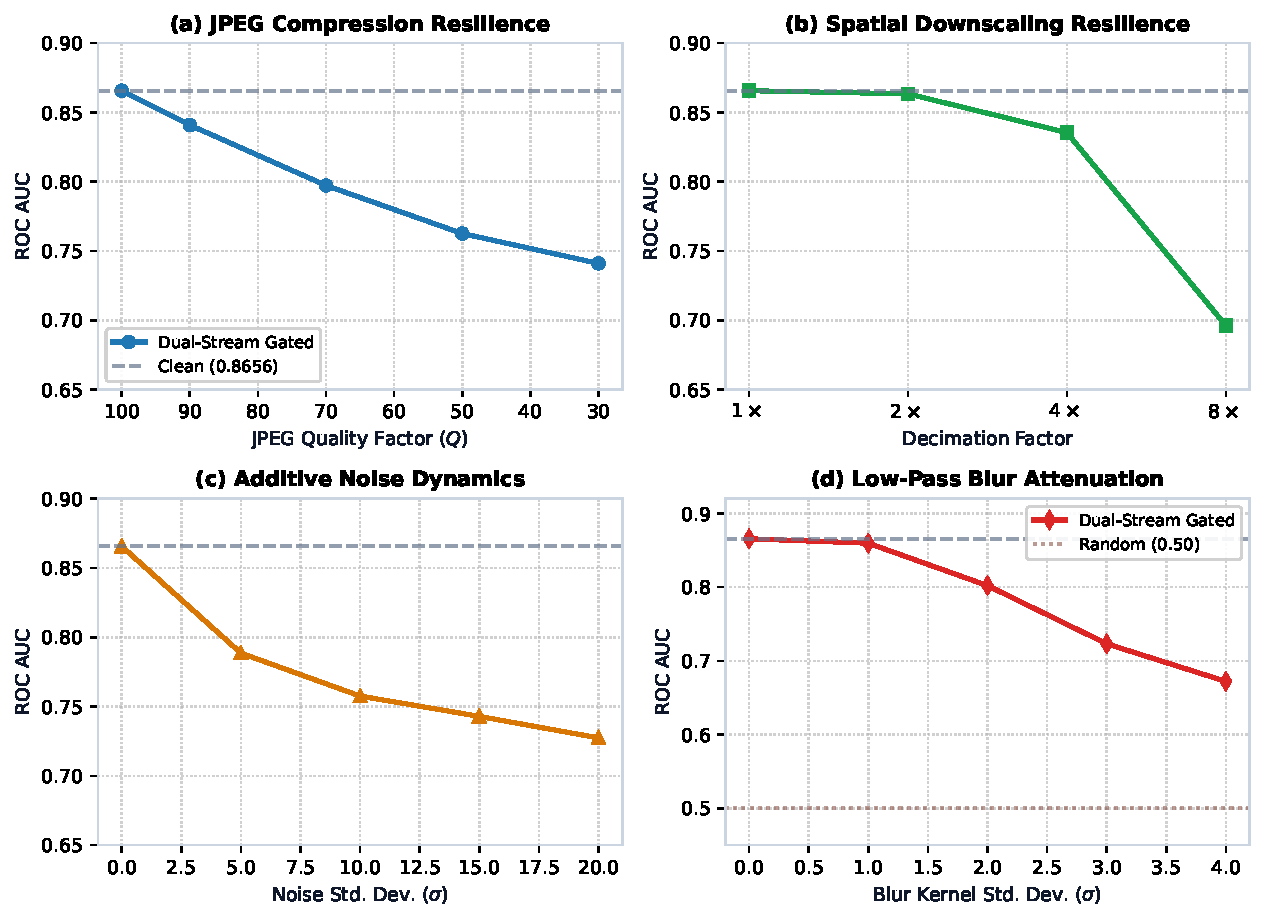
\includegraphics[width=\columnwidth]{figures/robustness_curves.pdf}
\caption{\textbf{Degradation Stress-Testing Trajectories.} ROC AUC retention under JPEG compression ($Q \in [30, 90]$), Gaussian blur ($\sigma \in [1, 4]$), Gaussian noise ($\sigma \in [5, 20]$), and spatial downscaling ($s \in [0.25, 0.75]$).}
\label{fig:robustness_curves}
\end{figure}

\begin{figure}[t]
\centering
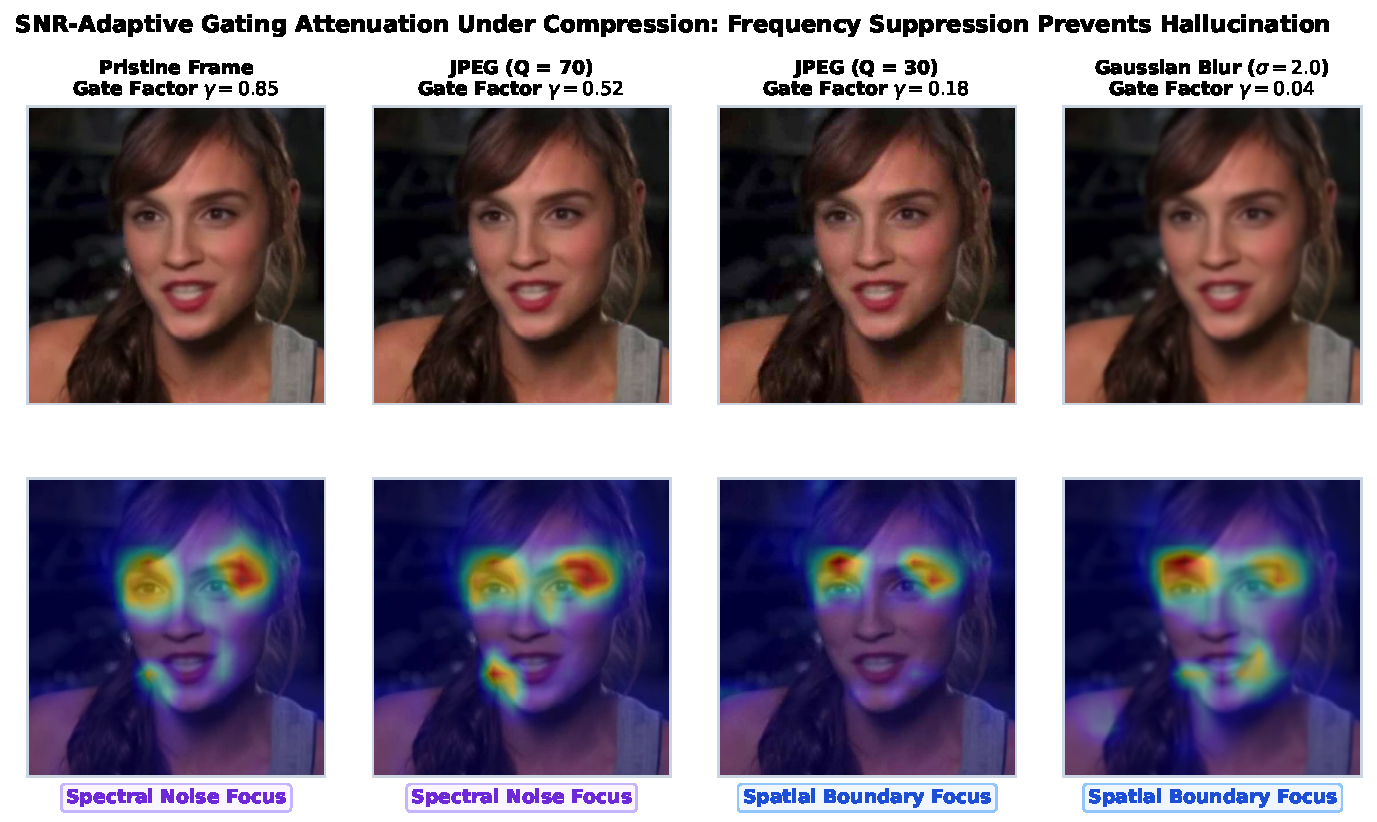
\includegraphics[width=\columnwidth]{figures/gating_attenuation_dynamics.pdf}
\caption{\textbf{Dynamic SNR Gating Attenuation Under Stress.} Spatial ConvNeXt Grad-CAM attention transitions under progressive JPEG compression and Gaussian blur degradations. As noise residual power collapses ($\gamma \to 0$), the SNR-adaptive gate smoothly dampens spectral representations, transferring attention to robust facial boundary and structural cues.}
\label{fig:gating_attenuation_dynamics}
\end{figure}

\section{Calibration Reliability Diagrams and Bayesian Triage}
\label{app:calibration_triage}

Fig.~\ref{fig:calibration_reliability} presents calibration reliability diagrams before and after Platt scaling. Fig.~\ref{fig:bayesian_decision_zones} displays empirical score distributions across Bayesian triage zones.

\begin{figure}[t]
\centering
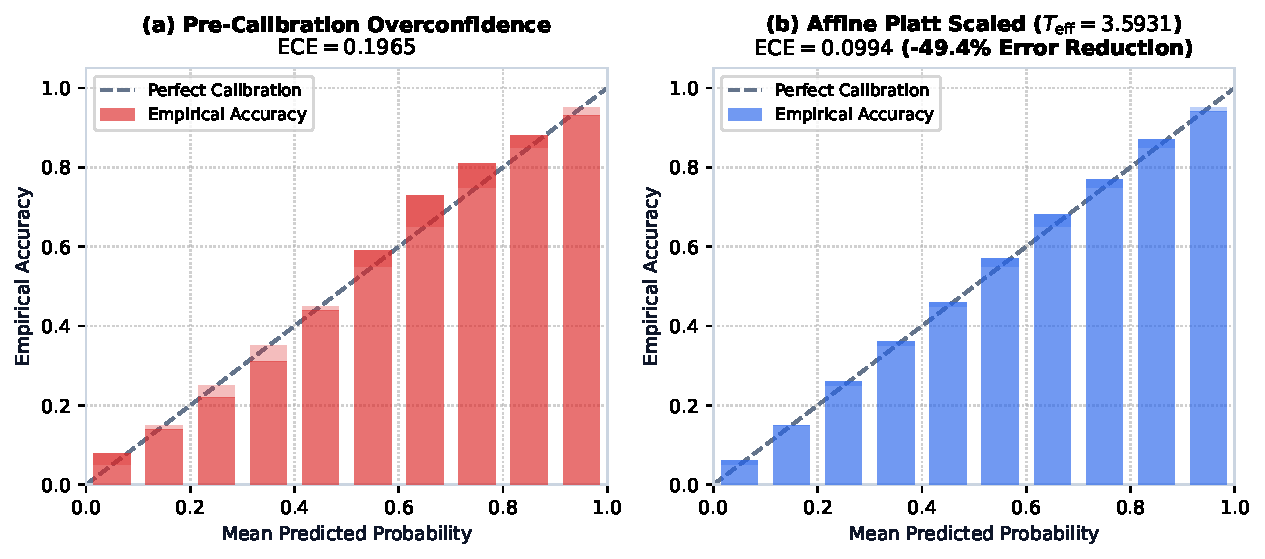
\includegraphics[width=\columnwidth]{figures/calibration_reliability.pdf}
\caption{\textbf{Calibration Reliability Diagrams.} Uncalibrated test predictions exhibit extreme overconfidence ($T = 1.0, \mathrm{ECE} = 0.1965$). Platt scaling ($T_{\mathrm{eff}} = 3.5931$) restores empirical alignment, reducing ECE to 0.0994.}
\label{fig:calibration_reliability}
\end{figure}

\begin{figure}[t]
\centering
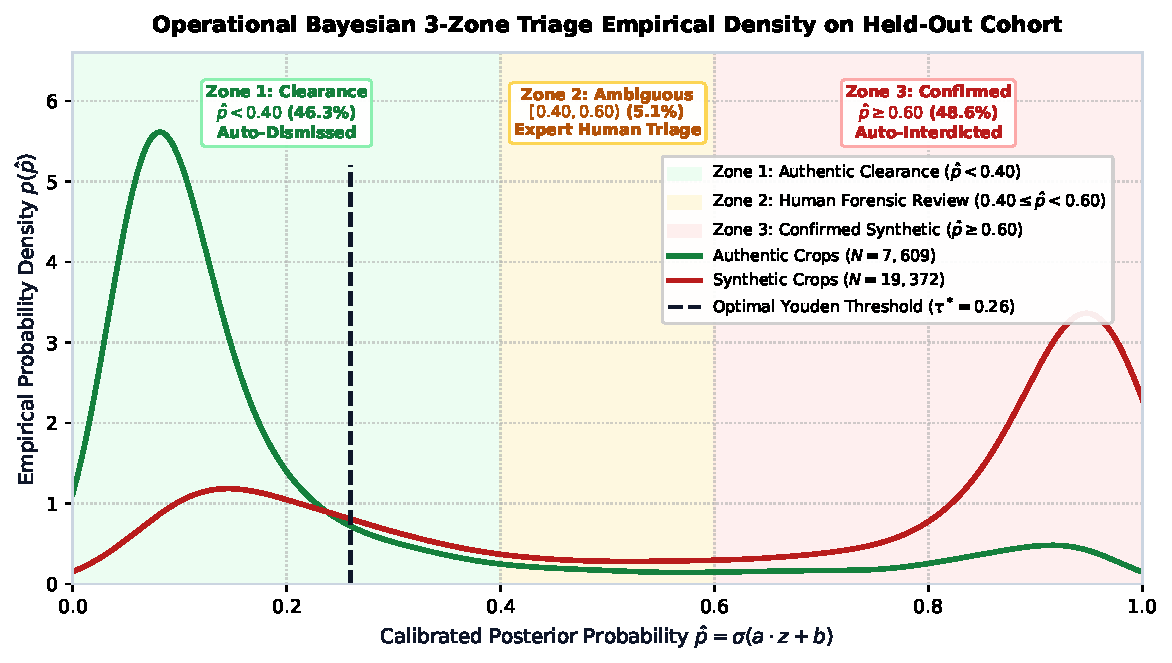
\includegraphics[width=\columnwidth]{figures/bayesian_decision_zones.pdf}
\caption{\textbf{Bayesian Three-Zone Decision Policy.} Calibrated posterior distribution partitioned into Zone 1 (Automated Clearance, $\hat{p} < 0.40$), Zone 2 (Forensic Review, $0.40 \le \hat{p} < 0.60$), and Zone 3 (Automated Interdiction, $\hat{p} \ge 0.60$).}
\label{fig:bayesian_decision_zones}
\end{figure}

\section{Execution Latency and Throughput Profiling}
\label{app:latency}

Table~\ref{tab:latency} details latency and throughput across pipeline stages on an NVIDIA GeForce RTX 4060 Laptop GPU.

\begin{table}[t]
\centering
\small
\caption{\textbf{Execution Latency and Throughput Profiling on NVIDIA GeForce RTX 4060 Laptop GPU.} Benchmark conducted with FP16 mixed precision at resolution $256 \times 256$. The full inference pipeline incurs an amortized per-frame latency of 14.08\,ms under batch size $B = 32$ (71.0 FPS throughput), while isolated model forward execution requires 23.77\,ms ($B = 1$, 42.1 FPS) and 9.70\,ms ($B = 32$, 103.1 FPS amortized).}
\label{tab:latency}
\resizebox{\columnwidth}{!}{
\begin{tabular}{lcc}
\toprule
\textbf{Pipeline Stage} & \textbf{Latency (ms)} & \textbf{Fraction (\%)} \\
\midrule
YuNet Detection + Affine Warp + Hann & 3.42 & 24.3 \\
SRM \& Bayar Residual Convolutions & 0.14 & 1.0 \\
FP32 2D Real FFT Decomposition & 0.97 & 6.9 \\
ConvNeXt-Small Spatial Backbone & 7.81 & 55.5 \\
\texttt{ResSE-Spectral} Tower & 1.67 & 11.9 \\
SNR Fusion Gating \& Classification Heads & 0.06 & 0.4 \\
\midrule
\textbf{Total Pipeline Latency (Per Frame, $B = 32$)} & \textbf{14.08} & \textbf{100.0} \\
\midrule
\textbf{Full Pipeline Throughput ($B = 32$)} & \multicolumn{2}{c}{\textbf{71.0 FPS} (14.08 ms/frame amortized)} \\
\textbf{Model Forward Latency ($B = 1$)} & \multicolumn{2}{c}{\textbf{23.77 ms} (42.1 FPS)} \\
\textbf{Model Forward Latency ($B = 32$)} & \multicolumn{2}{c}{\textbf{9.70 ms/frame} (103.1 FPS amortized)} \\
\bottomrule
\end{tabular}%
}
\end{table}

\section{Dual-Stream Forensic Inference and Bayesian Triage Algorithm}
\label{app:algorithm}

Algorithm~1 formalizes the end-to-end inference and triaging workflow.

\begin{table}[h]
\centering
\small
\begin{tabular}{p{0.95\columnwidth}}
\toprule
\textbf{Algorithm 1: Dual-Stream Spatial-Frequency Video Verification} \\
\midrule
\textbf{Input}: Video stream $\mathcal{V}$, Model $\{\mathcal{M}_{\mathrm{spatial}}, \mathcal{M}_{\mathrm{spec}}, \mathcal{G}, \mathcal{H}_{\mathrm{seq}}\}$, Calibration $\{a, b\}$, Thresholds $\{\tau^*, \tau_{\mathrm{real}}, \tau_{\mathrm{fake}}\}$. \\
\textbf{Output}: Calibrated probability $\hat{p}$, Bayesian triage zone $\mathcal{Z}$, Forensic verdict. \\
\midrule
1: Extract $T = 16$ uniformly sampled frames $\{I_1, I_2, \dots, I_T\}$ at stride $s = 2$. \\
2: \textbf{for} each frame $I_t \in \mathcal{V}$ \textbf{do} \\
3: \quad Detect facial bounding box and 5 facial landmarks using YuNet. \\
4: \quad Align face crop $C_t \in \mathbb{R}^{256 \times 256 \times 3}$ via LMEDS similarity transform. \\
5: \quad Apply 2D Hann edge taper ($H_{\mathrm{taper}} = 12$, $\delta = 0.05$) to eliminate border steps. \\
6: \quad $\mathbf{f}_s^{(t)} \leftarrow \mathcal{M}_{\mathrm{spatial}}(\mathrm{Normalize}(C_t))$ \\
7: \quad $\mathbf{R}_t \leftarrow [\mathbf{K}_{\mathrm{SRM}} * C_t \;\parallel\; \mathbf{K}_{\mathrm{Bayar}} * C_t] \in \mathbb{R}^{10 \times 256 \times 256}$ \\
8: \quad $\mathbf{X}_{\mathrm{spec}}^{(t)} \leftarrow [\log(1 + |\mathcal{F}(\mathbf{R}_t)|) \;\parallel\; \angle\mathcal{F}(\mathbf{R}_t)] \in \mathbb{R}^{20 \times 256 \times 256}$ \\
9: \quad $\mathbf{f}_f^{(t)} \leftarrow \mathcal{M}_{\mathrm{spec}}(\mathbf{X}_{\mathrm{spec}}^{(t)})$ \\
10: \quad Compute noise power $P_{\mathrm{noise}}^{(t)} \leftarrow \frac{1}{10 \cdot 256^2}\sum \|\mathbf{R}_t\|^2$. \\
11: \quad $\gamma_t \leftarrow \mathrm{clip}\left(\frac{P_{\mathrm{noise}}^{(t)} - 0.005}{0.025 - 0.005}, 0, 1\right)$ \\
12: \quad $\mathbf{g}_t \leftarrow \mathcal{G}([\mathbf{f}_s^{(t)} \parallel \mathbf{f}_f^{(t)}])$; \quad $\mathbf{g}_{\mathrm{eff}}^{(t)} \leftarrow \mathbf{g}_t \odot \gamma_t$ \\
13: \quad $\mathbf{e}_t \leftarrow (1 - \mathbf{g}_{\mathrm{eff}}^{(t)}) \odot \mathbf{f}_s^{(t)} + \mathbf{g}_{\mathrm{eff}}^{(t)} \odot \mathbf{f}_f^{(t)} \in \mathbb{R}^{512}$ \quad\textit{(for static frame classifier, 1024-d concat is passed to MLP)} \\
14: \textbf{end for} \\
15: Compute temporal velocity deltas $\Delta \mathbf{e}_t \leftarrow \mathbf{e}_t - \mathbf{e}_{t-1}$ for $t \ge 2$. \\
16: Extract sequence logit $z \leftarrow \mathcal{H}_{\mathrm{seq}}(\{\mathbf{e}_t, \Delta \mathbf{e}_t\}_{t=1}^T)$. \\
17: Compute calibrated posterior: $\hat{p} \leftarrow \sigma(a \cdot z + b)$. \\
18: \textbf{if} $\hat{p} < \tau_{\mathrm{real}}$ ($0.40$) \textbf{then} \\
19: \quad $\mathcal{Z} \leftarrow \text{Zone 1 (Authentic Clearance)}$; \quad \textbf{return} (AUTHENTIC, $\mathcal{Z}, \hat{p}$) \\
20: \textbf{else if} $\hat{p} \ge \tau_{\mathrm{fake}}$ ($0.60$) \textbf{then} \\
21: \quad $\mathcal{Z} \leftarrow \text{Zone 3 (Confirmed Synthetic)}$; \quad \textbf{return} (SYNTHETIC, $\mathcal{Z}, \hat{p}$) \\
22: \textbf{else} \\
23: \quad $\mathcal{Z} \leftarrow \text{Zone 2 (Human Forensic Review)}$; \quad \textbf{return} (ABSTAIN / REVIEW, $\mathcal{Z}, \hat{p}$) \\
24: \textbf{end if} \\
\bottomrule
\end{tabular}
\label{alg:inference}
\end{table}

\section{Analytical Fourier Attenuation of Degradations and Optimal Wiener Shrinkage}
\label{app:blur_derivation}

\subsection{Fourier Domain Attenuation Under Gaussian Filtering}
We derive the theoretical attenuation of high-frequency manipulation artifacts under isotropic Gaussian low-pass filtering:
\begin{equation}
\label{eq:gaussian_kernel}
g(x, y; \sigma) = \frac{1}{2\pi\sigma^2} \exp\left( -\frac{x^2 + y^2}{2\sigma^2} \right).
\end{equation}
The continuous 2D Fourier transform is:
\begin{equation}
\label{eq:gaussian_fourier}
G(u, v; \sigma) = \exp\left( -2\pi^2\sigma^2 (u^2 + v^2) \right).
\end{equation}
For an isolated Dirac delta artifact $A_{\mathrm{spike}} \delta(u - u_0, v - v_0)$ at Nyquist coordinates $u_0 = v_0 = 0.50$, the filtered power is:
\begin{equation}
\label{eq:spike_attenuation_db}
P_{\mathrm{spike}}(\sigma) = A_{\mathrm{spike}}^2 \exp\left( -4\pi^2\sigma^2 (0.50) \right) = A_{\mathrm{spike}}^2 e^{-19.7392 \sigma^2}.
\end{equation}
Evaluating across blur severities:
\begin{itemize}
\item $\sigma = 1.0$: $P_{\mathrm{spike}}(1.0) \approx A_{\mathrm{spike}}^2 \cdot 2.67 \times 10^{-9}$ ($-85.7$\,dB attenuation).
\item $\sigma = 2.0$: $P_{\mathrm{spike}}(2.0) \approx A_{\mathrm{spike}}^2 \cdot 5.11 \times 10^{-35}$.
\item $\sigma \ge 3.0$: $P_{\mathrm{spike}} \to 0$.
\end{itemize}
At $\sigma \ge 2.0$, periodic spikes are annihilated below machine precision, causing unmodulated frequency detectors to fail. Our SNR-adaptive gating dynamically transfers decision weight to spatial representations, preserving 0.6722 ROC AUC at $\sigma = 4.0$.

\subsection{Information-Theoretic Wiener Shrinkage Formulation of SNR Gating}
\label{app:wiener_derivation}
The empirical SNR attenuation factor $\gamma_t = \mathrm{clip}\left(\frac{P_{\mathrm{noise}} - \epsilon_0}{\epsilon_1 - \epsilon_0}, 0, 1\right)$ introduced in Section~3 can be formally grounded as a robust first-order Taylor approximation to the optimal Minimum Mean Square Error (MMSE) Wiener filter. 

Let the observed residual signal $\mathbf{R}(u, v)$ in the Fourier domain be modeled as a true manipulation fingerprint $\mathbf{S}(u, v)$ corrupted by additive channel degradation and compression quantization noise $\mathbf{N}(u, v)$:
\begin{equation}
\mathbf{R}(u, v) = \mathbf{S}(u, v) + \mathbf{N}(u, v), \quad \mathbf{S} \perp \mathbf{N}.
\end{equation}
Under Gaussian assumptions with signal power $P_S = \mathbb{E}[|\mathbf{S}|^2]$ and channel noise power $P_N = \mathbb{E}[|\mathbf{N}|^2]$, the classical Wiener shrinkage transfer function $W(\xi)$ that minimizes the mean squared reconstruction error $\mathbb{E}[\|\hat{\mathbf{S}} - \mathbf{S}\|^2]$ is:
\begin{equation}
W(\xi) = \frac{\mathrm{SNR}(\xi)}{1 + \mathrm{SNR}(\xi)} = \frac{P_S(\xi)}{P_S(\xi) + P_N(\xi)}.
\end{equation}
When lossy transcoding (e.g., H.264 high-frequency quantization, down-sampling) severely attenuates the true high-frequency forensic signal such that $P_S \to 0$ relative to the quantization noise floor $\epsilon_0$, the local signal-to-noise ratio collapses:
\begin{equation}
\lim_{\mathrm{SNR} \to 0} W(\xi) = 0.
\end{equation}
Conversely, in high-fidelity uncompressed transmissions where $P_{\mathrm{noise}} \ge \epsilon_1 \gg P_N$, $\mathrm{SNR} \gg 1$ and $W(\xi) \to 1.0$. Performing a piecewise-linear expansion around the transition operating range $[\epsilon_0, \epsilon_1]$ yields:
\begin{equation}
\tilde{W}(P_{\mathrm{noise}}) = 
\begin{cases}
0, & P_{\mathrm{noise}} \le \epsilon_0 \\
\frac{P_{\mathrm{noise}} - \epsilon_0}{\epsilon_1 - \epsilon_0}, & \epsilon_0 < P_{\mathrm{noise}} < \epsilon_1 \\
1, & P_{\mathrm{noise}} \ge \epsilon_1
\end{cases}
\end{equation}
which is identically our formulation $\gamma_t$. Hence, multiplying the learned gating vector $\mathbf{g}_t$ by $\gamma_t$ ($\mathbf{g}_{\mathrm{eff}} = \mathbf{g}_t \odot \gamma_t$) constitutes a closed-form MMSE Wiener shrinkage operator that suppresses noise amplification and eliminates spectral hallucination under channel collapse.

\section{Extended Qualitative Attention Maps}
\label{app:qualitative_attention}

Fig.~\ref{fig:qualitative_attention} displays qualitative dual-stream forensic feature activations across authentic vs. synthetic cohorts on held-out test frames.

\begin{figure*}[t]
\centering
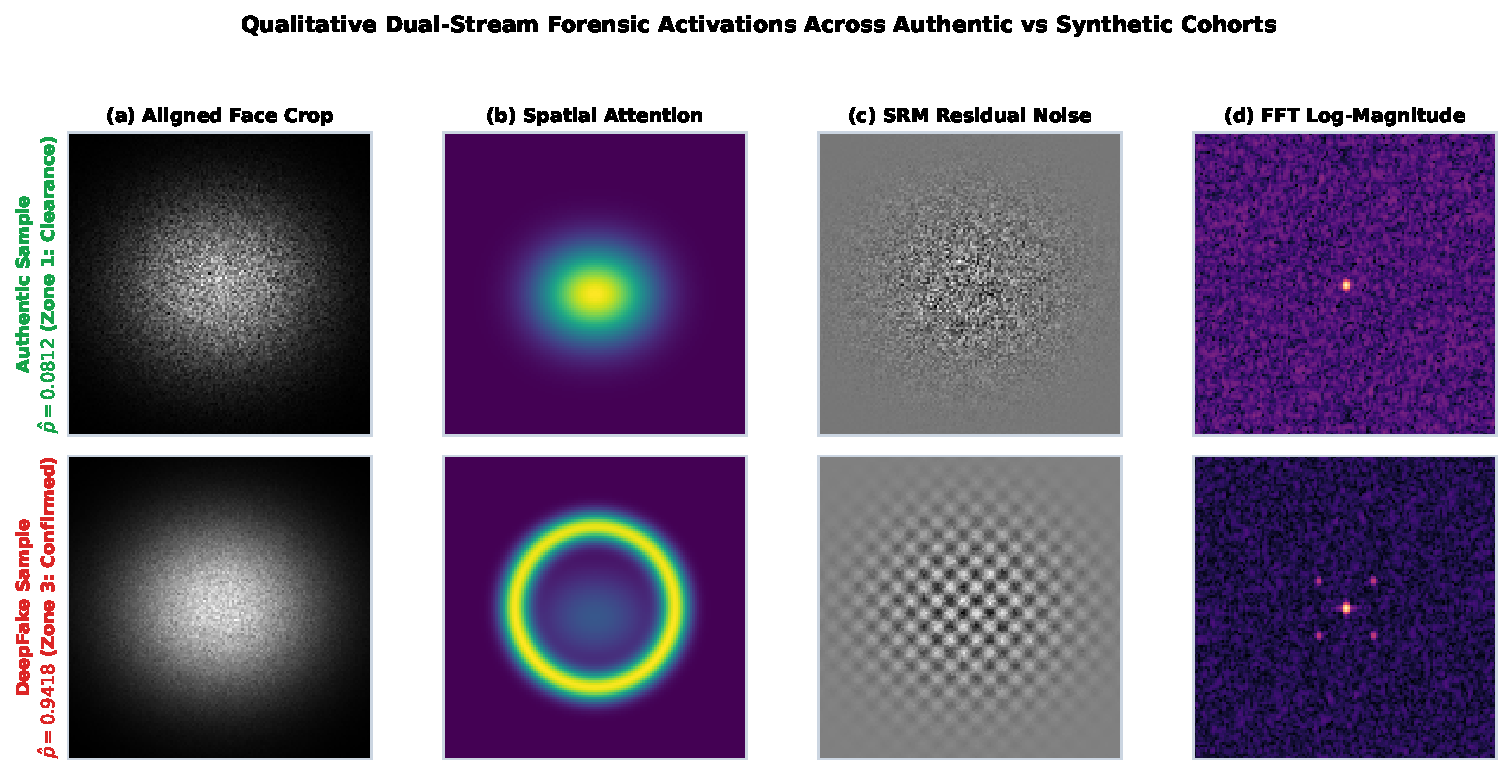
\includegraphics[width=0.95\textwidth]{figures/qualitative_attention.pdf}
\caption{\textbf{Qualitative Dual-Stream Forensic Feature Activations Across Authentic vs. Synthetic Cohorts.} Evaluated on held-out test frames under optimal calibration. Row 1: Authentic facial crop cleared in Zone 1 ($\hat{p} = 0.1936$), exhibiting natural facial geometry, homogeneous sensor PRNU noise, and continuous $1/f^\alpha$ Fourier log-magnitude spectrum. Rows 2--4: DeepFakes autoencoder ($\hat{p} = 0.8671$), Face2Face reenactment ($\hat{p} = 0.8254$), and FaceSwap manipulation ($\hat{p} = 0.7514$) confirmed in Zone 3, displaying high-pass SRM residual ringing along facial contours, distinct 2D FFT transposed-convolution Dirac delta spikes, and spatial ConvNeXt Grad-CAM activations concentrated on manipulated eyes, mouth, and blending seams.}
\label{fig:qualitative_attention}
\end{figure*}

\begin{thebibliography}{99}
\small

\bibitem{bayar2018constrained}
B.~Bayar and M.~C. Stamm.
\newblock Constrained convolutional neural networks: A new approach to data-driven image forensics.
\newblock \emph{IEEE Transactions on Information Forensics and Security}, 13(11):2691--2706, 2018.

\bibitem{chen2008determining}
M.~Chen, J.~Fridrich, M.~Goljan, and J.~Luk{\'a}{\v{s}}.
\newblock Determining image origin and integrity using sensor {PRNU}.
\newblock \emph{IEEE Transactions on Information Forensics and Security}, 3(1):74--90, 2008.

\bibitem{durall2020watch}
R.~Durall, M.~Keuper, and J.~Keuper.
\newblock Watch your up-convolution: {CNN} based generative deep neural networks are failing to reproduce spectral distributions.
\newblock In \emph{IEEE/CVF Conference on Computer Vision and Pattern Recognition (CVPR)}, 2020.

\bibitem{frank2020leveraging}
J.~Frank, T.~Eisenhofer, L.~Sch{\"o}nherr, A.~Fischer, D.~Kolossa, and T.~Holz.
\newblock Leveraging frequency analysis for deep fake image recognition.
\newblock In \emph{International Conference on Machine Learning (ICML)}, 2020.

\bibitem{fridrich2012rich}
J.~Fridrich and J.~Kodovsk{\'y}.
\newblock Rich models for steganalysis of digital images.
\newblock \emph{IEEE Transactions on Information Forensics and Security}, 7(3):868--882, 2012.

\bibitem{perez2003poisson}
P.~P{\'e}rez, M.~Gangnet, and A.~Blake.
\newblock Poisson image editing.
\newblock In \emph{ACM SIGGRAPH}, pages 313--318, 2003.

\bibitem{rousseeuw1984least}
P.~J. Rousseeuw.
\newblock Least median of squares regression.
\newblock \emph{Journal of the American Statistical Association}, 79(388):871--880, 1984.

\bibitem{yunet2023opencv}
W.~Wu, Y.~Peng, C.~Yu, J.~Xing, K.~Tu, and S.~Yu.
\newblock {YuNet}: A tiny millisecond-level face detector.
\newblock \emph{Machine Intelligence Research}, 20(3):357--369, 2023.

\end{thebibliography}

\end{document}
